\def\nodesize{1.0cm}
\tikzstyle{neuron}=[circle, draw=black, minimum size=\nodesize]
\tikzstyle{dots}=[draw=none, scale=2, text height=0.333cm, execute at end node=$\vdots$]

\begin{figure}[!htp] %place it here (h)
  \centering
  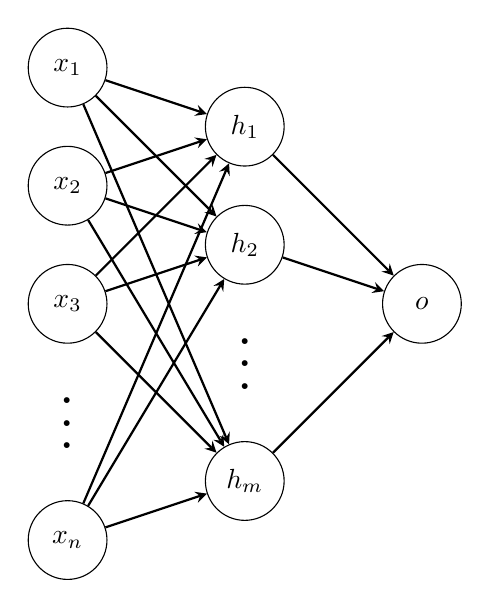
\begin{tikzpicture}[x=1.5cm, y=1.5cm, >=stealth] % >=stealth arrow style
    % input nodes
    \foreach \m [count=\y] in {1,2,3,dots,n} 
    {
      \ifnum\y=4
      \node [\m/.try] at (0,-\y) {};
      \else
      \node [neuron] (input-\m) at (0,-\y) {$x_\m$};
      \fi
    }
    % hidden nodes
    \foreach \m [count=\y] in {1,2,dots,m} 
    {
      \ifnum\y=3
      \node [\m/.try] at (1.5, -\y - 0.5) {};
      \else
      \node [neuron] (hidden-\m) at (1.5, -\y - 0.5) {$h_\m$};
      \fi
    }

    % output node
    \node [neuron] (output) at (3, -3) {$o$};

    % activation function
    % \node [neuron] (activation) at (3.0, -3) {$g$};

    % input-hidden connections
    \foreach \m [count=\y] in {1,2,3,n}
    \foreach \n [count=\y] in {1,2,m}
    % above moves the text higher depending on the orientation of the line
    \draw [thick, ->] (input-\m) -- (hidden-\n) 
    node[above=4pt*abs(3 - \y), pos=0.45, scale=0.9] {};

    % input-hidden connections
    \foreach \m [count=\y] in {1,2,m}
    % above moves the text higher depending on the orientation of the line
    \draw [thick, ->] (hidden-\m) -- (output) 
    node[above=4pt*abs(3 - \y), pos=0.45, scale=0.9] {};

  \end{tikzpicture}
  \caption{Schematizzazione del Multi Layer Perceptron: in Figura è mostrata
    una rete neurale con $n$ valori di input, un singolo hidden layer con $m$
    neuroni e un solo output. Si noti che non si è limitati ad usare un solo
    neurone di output. Sono omessi per chiarezza i parametri del modello e le
    funzioni di attivazione, riassunte in questo caso all'interno di ogni
    neurone.}
  \label{fig:mlp}
\end{figure}
